\section{Experiments}
\label{experiments_section}
This section shows the performance of our method for both the {\em supervised setting}, where we see examples of the specific level in both training and test time, and the {\em unseen setting}, where we are testing on new levels, not seen during training.
We will compare the benefits of the different components of our approach and show an example solution produced by our method.

\subsection{Benefits of different components of our approach}
As the base method we use the off-the-shelf \maskrcnn approach (``Vanilla \maskrcnn''), which has a low accuracy even on simple \alphapack levels.
To improve over this baseline, we have introduced several additional components, namely, ``Automatic point detection'', ``History channel'', ``4+ Stage training'', ``Intersection degeneration rules'', and ``On-the-fly data generation'' (see Section~\ref{mrcnn_components}).
Table~\ref{components_performance} compares their cumulative benefits.
These components are crucial for solving levels in advanced level packs, e.g., the Gamma level pack, which could not be solved without the Intersection degeneration rules.

\begin{table}[!htb]
    \centering
    \begin{tabular}{p{48mm}|
    m{11mm}m{11mm}m{11mm}m{11mm}m{11mm}m{11mm}
    }
     Component / Level pack & \alphapack & \betapack & \gammapack & \deltapack & \epsilonpack & \zetapack  \\
     \hline
     Vanilla \maskrcnn~\cite{maskrcnn} & 71.0 & - & - & - & - & - \\
     + Automatic point detection & 95.1 & - & - & - & - &  - \\
     + History channel & 98.1 & 69.3 & - & - & - & -  \\ 
     + 4+ Stage training & 91.7 & 82.3 & - & - & - & - \\
     + Intersection degeneration rules & 91.7 & 82.3 & 79.9 & 73.5 &  - &  - \\
     + On-the-fly data generation & {\bf 98.7} & {\bf 96.2} & {\bf 97.8} & {\bf 99.1} & {\bf 92.8} & {\bf 95.7}\\
    \end{tabular}
    \caption{Performance of the base method (Vanilla \maskrcnn) together with the additional components of our approach. The Performance is evaluated on Euclidea level packs with increasing difficulty (from \alphapack to \zetapack). We trained a separate model for every level in each level pack and evaluated the model on 500 new  instances of that level.
    The table presents the accuracy averaged across all levels in each level pack.
    The components are applied to the base method (Vanilla \maskrcnn) in an additive manner.
    For example, the 4+ Stage training includes all previous components, i.e.,~Automatic point detection and History channel.
    A description of the different components is given in Section \ref{mrcnn_components}.}
    \label{components_performance}
    \vspace{-3.3em}
\end{table}


\begin{figure}[!htb]
    \centering
    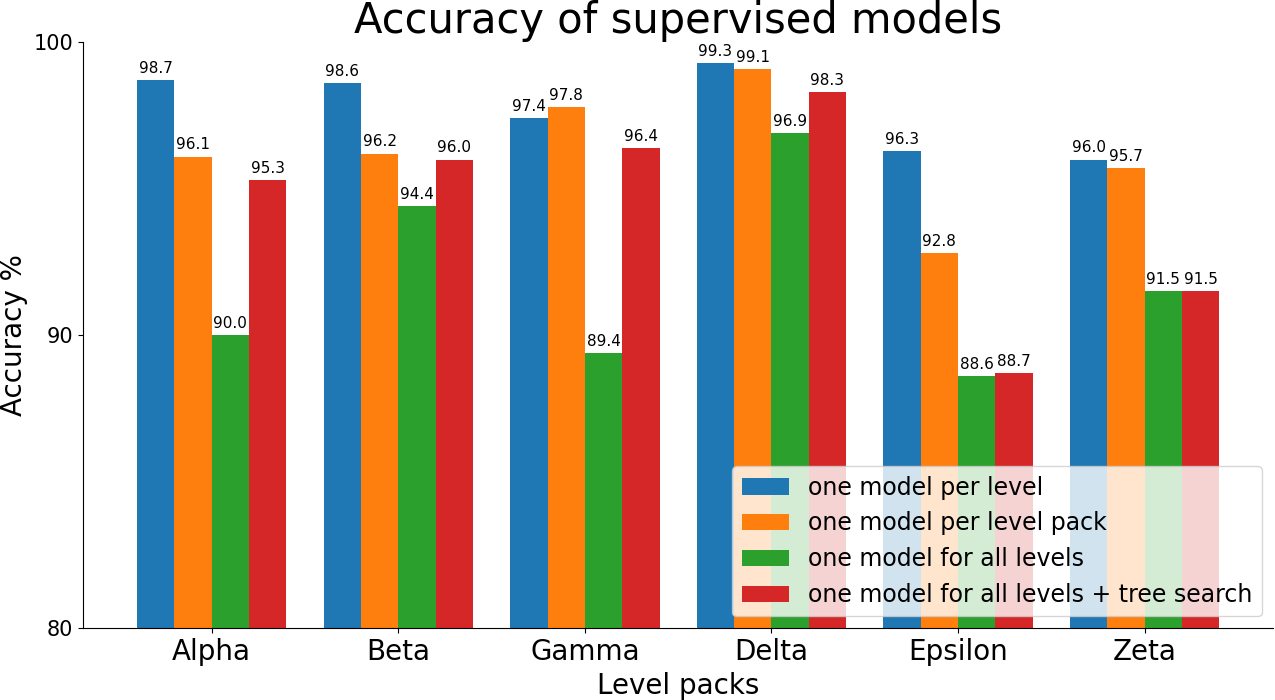
\includegraphics[width=0.88\textwidth]{img/acc_barplot_with_t_search.png}
    \caption{Accuracy of our approach on Euclidea level packs Alpha to Zeta.
    The model uses all components from Table \ref{components_performance}.
    We compare four approaches: one model per level (blue), one model per level pack (orange), one model for all levels (green), and one model for all levels with hypothesis tree search (red). All were evaluated on 500 instances of each level and the accuracy was averaged across all levels in each level pack.
    }
    \label{final_results}
    \vspace{-2em}
\end{figure}
\subsection{Evaluation of the supervised learning approach}

We evaluated our method on the first six level packs of Euclidea with various training setups. The results (see Fig.~\ref{final_results}) show that models specialized to individual level packs (``one model per level pack'') or even levels (``one model per level'') have better accuracy than a single, more general model for multiple levels/packs (``one model for all levels''). We also investigate the benefits of using our tree search procedure (see Section~\ref{hypotheses_tree_search}) instead of using only the most confident hypothesis, as in the supervised setting. We find the tree search improves the accuracy, especially on \alphapack and \gammapack level packs, by searching the space of possible candidate solutions for each step of the construction.
\subsection{Evaluation on unseen problems}

To evaluate performance on unseen levels, we use the leave-one-out (LOO) evaluation.
In our setup, \emph{LOO levels} evaluates, e.g., level \textit{Alpha-01} using models trained on each of the other \alphapack levels, whereas \emph{LOO packs} evaluates, e.g., each \alphapack level using models trained on level packs \betapack, \gammapack, \deltapack, \epsilonpack, and \zetapack.
Table~\ref{tab:loo_eval} compares the LOO evaluation and the supervised approach, both with the hypothesis tree search, for level pack \alphapack.
We ran a similar evaluation for all 6 levels packs and were able to solve 30 out of 68 levels using \emph{LOO levels} and 31 out of 68 levels using \emph{LOO packs}.
The results show that our method can solve many levels unseen during the training, although some levels remain difficult to solve.
\label{eval_of_unseen_levels}
\begin{table}[!htb]
    \centering
    \setlength{\tabcolsep}{12pt}
    \begin{tabular}{l|ccc}
     \alphapack levels & LOO levels & LOO packs& supervised\\
     \hline
     01 T1 Line & 40.0 & 10.0 & 85.0\\
     02 T2 Circle & 5.0 & 45.0 & 100.0\\
     03 T3 Point & 100.0 & 90.0 & 100.0\\
     04 TIntersect & 100.0 & 100.0 & 99.0\\
     05 TEquilateral & 50.0 & 70.0 & 100.0\\
     06 Angle60 & 55.0 & 100.0 & 94.0\\
     07 PerpBisector & 35.0 & 100.0 & 99.0\\
     08 TPerpBisector & 0.00 & 100.0 & 75.0\\
     09 MidPoint & 5.0 & 60.0 & 100.0\\
     10 CircleInSquare & 0.00 & 100.0 & 87.0\\
     11 RhombusInRect & 25.0 & 40.0 & 99.0\\
     12 CircleCenter & 10.0 & 0.00 & 100.0\\
     13 SquareInCircle & 0.00 & 10.0 & 100.0\\
     \hline
     Average & 42.5 & 63.4 &95.3\\
\end{tabular}
    \caption{Leave-one-out evaluation on the Alpha levels.
    Completion accuracy of the leave-one-out evaluation across levels within a level pack (LOO levels), across level packs (LOO packs), and, for comparison, our best supervised model trained to solve the first six Euclidea level packs (\alphapack-\zetapack); the tree search was used in all three cases.
    The leave-one-out evaluation was performed on 20 instances of each level, while the supervised model was evaluated on 500 instances of each level. Using models from all level packs except Alpha (LOO packs) works better than using models trained only on other levels of the Alpha level pack (LOO levels). This is likely because models in the ``LOO packs" set-up have seen a larger set of different constructions.
}
    \label{tab:loo_eval}
    \vspace{-2em}
\end{table}

\newpage
\subsection{Qualitative example}

Fig.~\ref{fig:Epsilon12_example} shows a step-by-step walk-through construction of an advanced Euclidea level.

\begin{figure}[!h]
     \centering
     \begin{subfigure}[t]{0.32\textwidth}
         \centering
         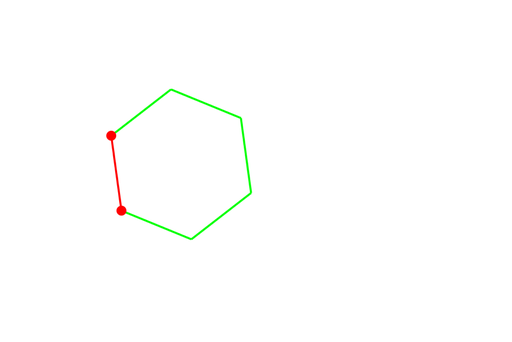
\includegraphics[width=\textwidth]{img/Epsilon-12_example/input_image0.png}
         \caption{Input}
         \label{fig:Epsilo12_example_input}
     \end{subfigure}
     \hfill
     \begin{subfigure}[t]{0.32\textwidth}
         \centering
         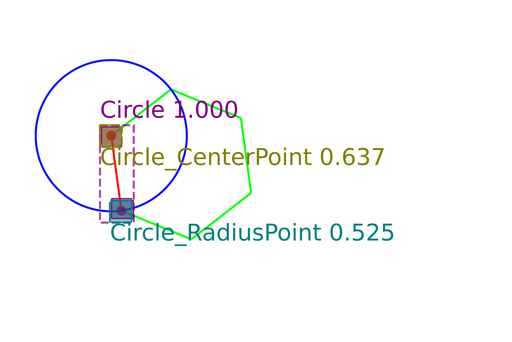
\includegraphics[width=\textwidth]{img/Epsilon-12_example/output_image0.png}
         \caption{Step 1: Circle tool}
         \label{fig:Epsilon12_example_step1}
     \end{subfigure}
     \hfill
     \begin{subfigure}[t]{0.32\textwidth}
         \centering
         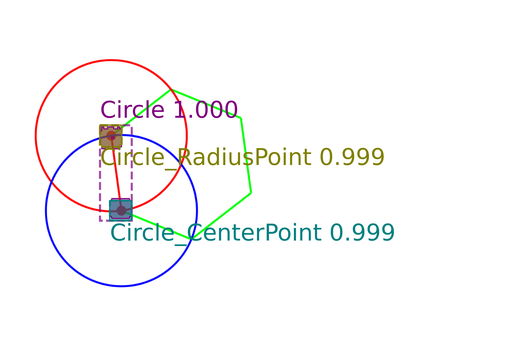
\includegraphics[width=\textwidth]{img/Epsilon-12_example/output_image1.png}
         \caption{Step 2: Circle tool}
         \label{fig:Epsilon12_example_step2}
     \end{subfigure}
     \hfill
     \begin{subfigure}[t]{0.32\textwidth}
         \centering
         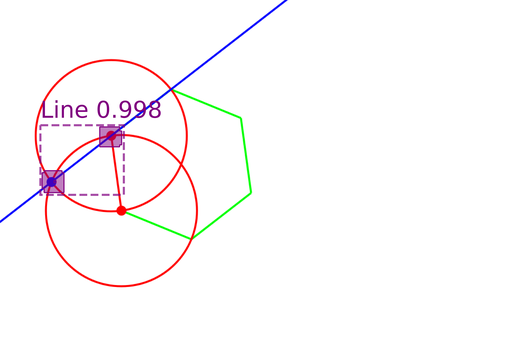
\includegraphics[width=\textwidth]{img/Epsilon-12_example/output_image2.png}
         \caption{Step 3: Line tool}
         \label{fig:Epsilon12_example_step3}
     \end{subfigure}
     \hfill
     \begin{subfigure}[t]{0.32\textwidth}
         \centering
         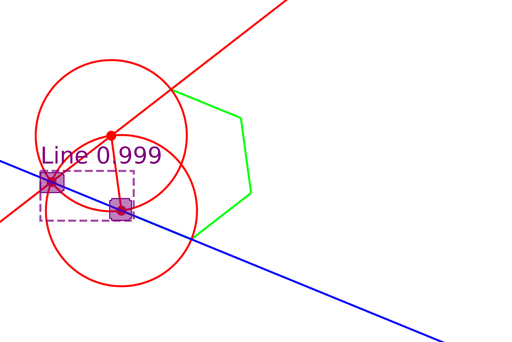
\includegraphics[width=\textwidth]{img/Epsilon-12_example/output_image3.png}
         \caption{Step 4: Line tool}
         \label{fig:Epsilon12_example_step4}
     \end{subfigure}
     \hfill
     \begin{subfigure}[t]{0.32\textwidth}
         \centering
         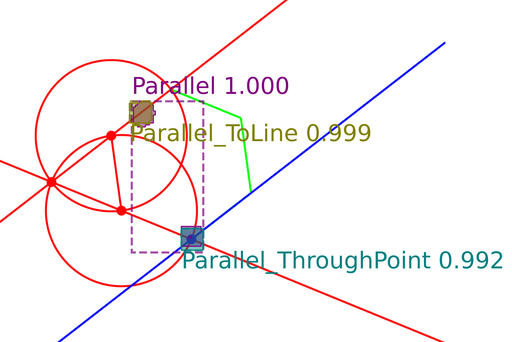
\includegraphics[width=\textwidth]{img/Epsilon-12_example/output_image4.png}
         \caption{Step 5: Parallel tool}
         \label{fig:Epsilon12_example_step5}
     \end{subfigure}
     \hfill
     \begin{subfigure}[t]{0.32\textwidth}
         \centering
         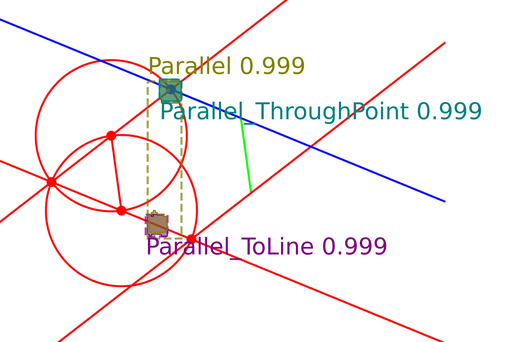
\includegraphics[width=\textwidth]{img/Epsilon-12_example/output_image5.png}
         \caption{Step 6: Parallel tool}
         \label{fig:Epsilon12_example_step6}
     \end{subfigure}
     \hfill
     \begin{subfigure}[t]{0.32\textwidth}
         \centering
         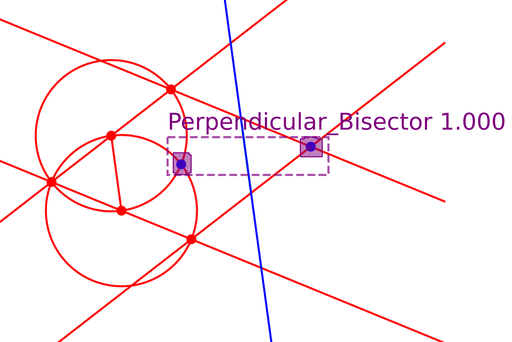
\includegraphics[width=\textwidth]{img/Epsilon-12_example/output_image6.png}
         \caption{Step 7: Perpendicular tool}
         \label{fig:Epsilon12_example_step7}
     \end{subfigure}
     \hfill
     \begin{subfigure}[t]{0.32\textwidth}
         \centering
         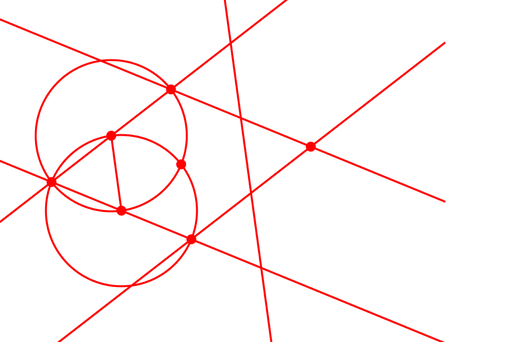
\includegraphics[width=\textwidth]{img/Epsilon-12_example/input_image7.png}
         \caption{Construction finished}
         \label{fig:Epsilon12_example_fin}
     \end{subfigure}
     \hfill
     
        \caption{Example construction of Euclidea level \textit{Epsilon-12} (construct a regular hexagon by the side).
        (a) Initial configuration of the problem.
        (b-h) Seven construction steps, including \maskrcnn detections, and an object proposed to construct in each step.
        (i) Final construction step, level solved.
        Red denotes the current state of the construction, green the remaining goal,
        blue the geometric primitive proposed by the detection,
        and other colors
        the prediction masks, bounding boxes, class names, and scores for the next predicted action.
        More examples can be found in the supplementary material available at the project webpage~\cite{project-page}.
        }
        \label{fig:Epsilon12_example}
\end{figure}

\paragraph{\textbf{Connections between levels.}}
\label{connections}
From the leave-one-out evaluation, we can also observe which levels are similar.
We denote that level $X$ is \emph{connected} to level $Y$ if a model trained for $Y$ contributes with a hypothesis to a successful construction during the inference for level $X$.
Note that this relation is not symmetric, e.g.,~when $X$ is connected to $Y$, then $Y$ is not necessarily connected to $X$.
We run the hypothesis tree search during the leave-one-out evaluation and obtain connections in the following way: If the search is successful, we collect all models that contributed to the solution in the final backtracking of the search.
The connections for all levels in the level pack Alpha are shown in Fig.~\ref{connection_graph}.



\begin{figure}[htb!]
    \centering
    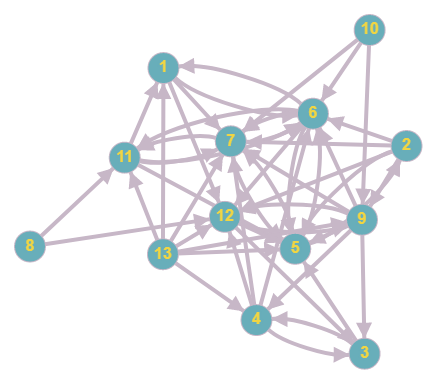
\includegraphics[width=0.4\textwidth]{img/connection_graph.png}
    \caption{
    \small Connection graph created during the leave-one-out evaluation of the Alpha level pack using models for individual levels. Models trained on 
    more difficult levels (indicated by higher numbers) often help construct easier levels (lower numbers). For example, level 13 could not be solved (has no incoming connections), but its predictions were used for solution of levels 1, 4, 5, 7, 9, 11, 12. Our method can often construct simpler tasks based on more complex constructions. However, combining multiple simple tasks into a complex construction remains a challenge.
    }
    \label{connection_graph}
\end{figure}
